\section{$\lgname$ case studies}

The $\lgname$ simulator provides the user a way to test, debug and demonstrate the application program logic, with custom dynamics models without incurring the cost of hardware deployment. In this section, we present some case studies to demonstrate some important capabilities of $\lgname$ using simulations. 
\subsection{Platooning}
%end to end
\label{sec:platooning}
In this program, the system handles automated vehicles moving in a platoon, by communicating through shared variables. The goal of this program is to maintain at least a \emph{safe} distance between any two consecutive cars. The first car (highest pid) sets its acceleration to 2 or -2 every 10 rounds. The motion controller for the car has bounds on highest and lowest velocities allowed. Every other car with pid $i$ sets the actuator for its acceleration based on its distance from the car with pid $i+1$. The cars communicate through the \emph{allread} variable $\mathit{pos}$, which they update every time they execute the event \emph{SetAcc}, or, as the semantics dictates, every $\delta$ time units.

\begin{figure}[ht!]
    \noindent
    \begin{center}
        \scriptsize
        \two{0.4}{0.6}
        {\lstinputlisting[language=xyzNums,firstline=1,lastline=21,frame=none]{code/platooning2.tex}}
        {\lstinputlisting[language=xyzNums,firstline=22,frame=none,firstnumber=22]{code/platooning2.tex}}
    \end{center}
    \caption{$\lgname$ program for robot $i$ in a Platoon to adjust its $x$ acceleration accordingly .}
    \label{fig:platooningapp}
\end{figure}


\reffig{platoon} shows the resulting $x$ vs $\mathit{time}$ plots for different values of $\delta$, or the duration of the environment transition in \reffig{platoon}. These plots were saved directly from the simulator, and the blue progress bar on the top of the plot shows how far in the current simulation this plot is generated.

\begin{figure}[h!]
\begin{minipage}{0.5\textwidth}
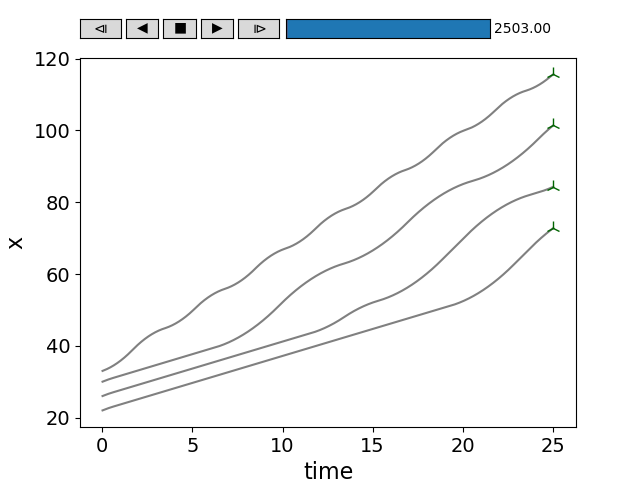
\includegraphics[width=.5\textwidth]{figs/braking_acc.png}}\hfill%
%\includegraphics[width=.3\textwidth]{figs/Platooning_2.png}}\hfill%
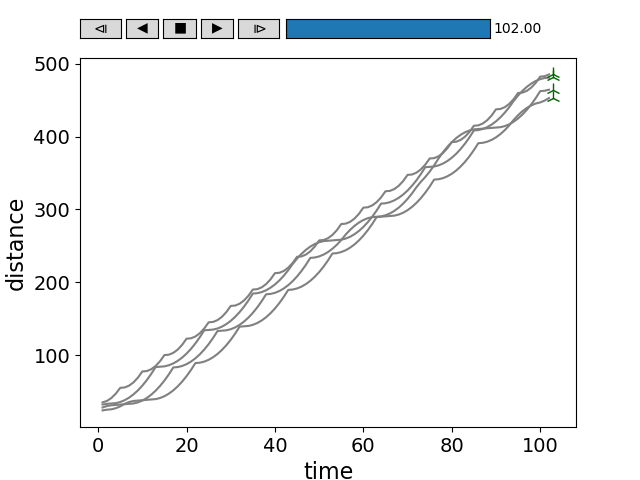
\includegraphics[width=.5\textwidth]{figs/braking_bad.png}
\end{minipage}%
	\caption{\small {Platoon of four cars. \emph{Left} for $\delta = 0.01$, the cars eventually get to safe separations, while reacting to the first car changing its acceleration periodically} and \emph{Right} for $\delta = 0.1$, this shows an unsafe execution where the simulation stops upon a collision.}
\label{fig:platoon}
\end{figure}

%FIGURE OUT THE VERIFICATION. 
 A \emph{correct} program should ensure that at no point, the separation along the $x$-axis between two of agents is less than the required safe distance.  Note, that the variable $\emph{safedist}$ needs to be set to higher than the actual required separation to account for reacting to the previous vehicle updating its $\mathit{pos}$ value, depending on how long the sampling parameter $\delta$ is. We verified using our bounded model checker, that \emph{Platoon} (\reffig{platooningapp}) was indeed safe (for four cars) frequent position sampling, i.e, when $\delta$ is small enough and the variable $\emph{pos}$ is updated frequently, and unsafe otherwise.  \reffig{platoon}(Right) shows the $x$ vs $\mathit{time}$ when the cars react too slowly.


\subsection{Formation}
%portability
\label{sec:formation}
We used $\lgname$ to do implement some standard robotics \emph{formation} programs. The \emph{Lineform} app uniformly lines up the positions of  agents between the robots with the minimum and maximum $pid$. For the non-extremal agents, it sets the target way-point as the mid-point of the position of its neighbors. This type of linear update rule of is an example of hundreds of textbook algorithms for distributed consensus, rendezvous, optimization, swarm flocking, pattern formation~\cite{Tsitsiklis:1986,Blondel,Magnusbook2010} that are directly translated to working implementations using $\lgname$. The mathematical description of the algorithm found in control theory textbooks is shown on the right. 

\begin{figure}[ht!]
	\label{fig:lineform}
	\noindent
	\begin{center}
		\scriptsize
		\two{0.4}{0.6}
		{\lstinputlisting[language=xyzNums,frame=none]{code/lineform.tex}}
		{ \vspace{0.1in}
                        $x_{t+1} = Ax_{t}$, where \\
			$x_0$: vector of initial position of agents, \\
			$x_{t}$: position vector at time $t$, and \\
		        $A$: is the \emph{transition matrix}, for lineform  \\
                  
			$A  = \left[ \begin{array}{ccccc}
			0 & 0 & 0 & 0 & 0\\
			\frac{1}{2} & 0 & \frac{1}{2} & 0 & 0\\
			0 & \frac{1}{2} & 0 & \frac{1}{2} & 0  \\
			0 & 0 & \frac{1}{2} & 0 & \frac{1}{2} \\
			0 & 0 & 0 & 0 & 0\\			
			\end{array}\right]$
			}
	\par
        
	\end{center}
	\caption{\small $\lgname$ program for line formation ({\em Left}) and its mathematical counterpart in robotics and control textbooks ({\em Right}).}
\end{figure}

The shared \emph{allread} variable $p$ (Line\ref{lineformp}) is used by the agents to communicate their position to the other robots. The function \emph{midpoint} is a part of the library functions provided for the data type \emph{pos}; where $$\mathit{midpoint}(p_1,p_2,\ldots,p_n) = pos(\frac{\Sigma_n p_i.x}{n},\frac{\Sigma_n p_i.y}{n},\frac{\Sigma_n p_i.z}{n}) $ \rg{We provide the $\lgname$ definitions of all auxiliary library functions used in the code in the appendix \ref{auxfuncs}.}
\iffalse

\reffig{lineformplots} shows two screenshots of the simulation of this appp with 5 robots forming a line. 

\begin{figure}[h!]
\begin{minipage}{0.5\textwidth}
%\includegraphics[width=.3\textwidth]{figs/Platooning_2.png}}\hfill%
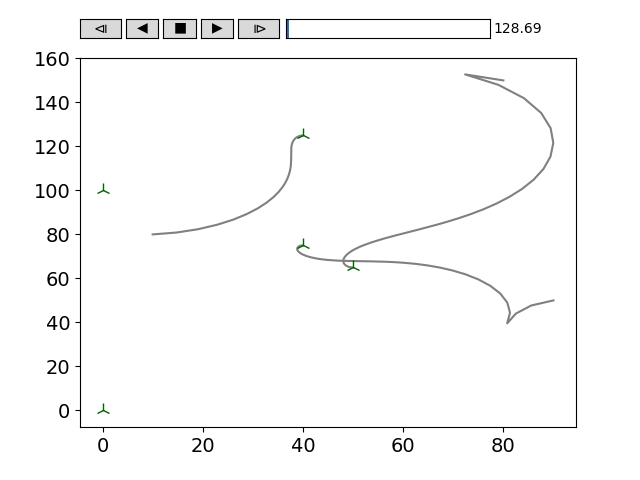
\includegraphics[width=.5\textwidth]{figs/lineform2.png}\hfill
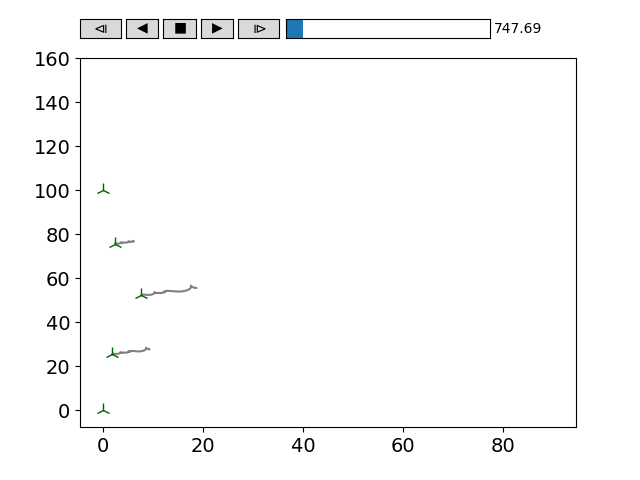
\includegraphics[width=.5\textwidth]{figs/lineform3.png}}\hfill%
%\includegraphics[width=.3\textwidth]{figs/Platooning_2.png}}\hfill%
\end{minipage}%
\caption{$x$ vs $y$ plots for Lineform. The grey trails represent the positions of the agents in the last 150 time steps.}
\label{fig:lineformplots}
\end{figure}
\fi
We updated the Lineform app with a neighbor relation, to create the \emph{Squareform} app as shown in \reffig{squareform}. The code defines a local variables $nbrs$ which is a static list of list of integers, where the $i$th element is a list of the $\mathid{pid}$s of the neighbors of the agent with $\mathit{pid}$ $i$. It also defines a list of integers called $\mathit{corners}$ which contains the $\mathit{pid}$s of agents which should be at the corners of the square. If the agent $pid$ is not in the list, then it moves to the mid point of all its neighbors. 

\begin{figure}[ht!]
    \noindent
    \begin{center}
        \scriptsize
        \two{0.4}{0.6}
        {\lstinputlisting[language=xyzNums,firstline=1,lastline=10,frame=none]{code/shapeform.tex}}
        {\lstinputlisting[language=xyzNums,firstline=11,frame=none,firstnumber=11]{code/shapeform.tex}}
    \end{center}
    \caption{$\lgname$ program for robot $i$ in a Platoon to adjust its $x$ acceleration accordingly .}
    \label{fig:platooningapp}
\end{figure}

\reffig{shapeplots} shows two screenshots of the 3d-simulation for the \emph{Shapeform} app with 25 agents. The agents eventually form a square along the plane specified by the four fixed end agents. 

\begin{figure}[h!]
\begin{minipage}{0.5\textwidth}
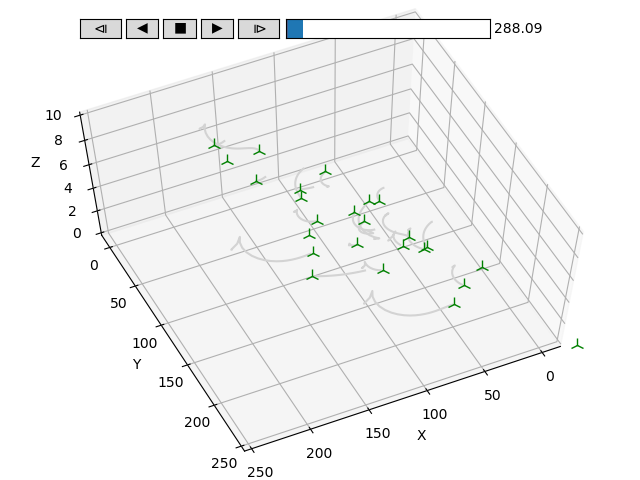
\includegraphics[width=.5\textwidth]{figs/formation1.png}\hfill
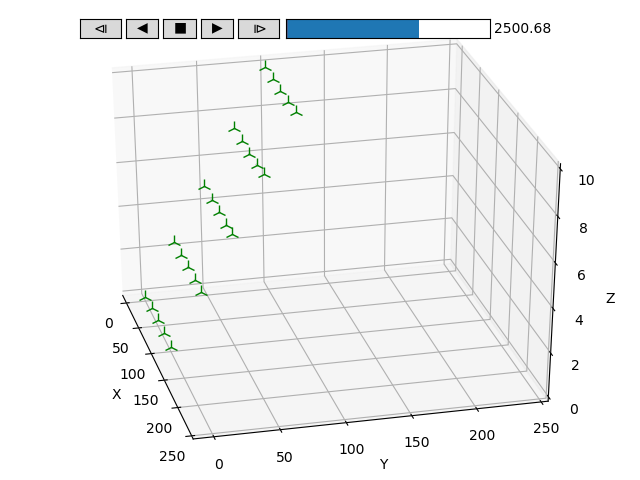
\includegraphics[width=.5\textwidth]{figs/formation5.png}}\hfill%
%\includegraphics[width=.3\textwidth]{figs/Platooning_2.png}}\hfill%
\end{minipage}%
\caption{$x$ vs $y$ vs $z$ plots for shapeform. The grey trails represent the positions of the agents in the last 150 time steps.}
\label{fig:shapeformplots}
\end{figure}

\subsection{Task}

 \reffig{taskapp} shows the distributed task allocation application written in $\lgname$. Distributed task allocation is challenging as it involves mutual exclusion as well as construction of de-conflicted  paths. Tasks can be abstractions for real location-based objectives like package delivery, surveillance, or fire-fighting. $\lgname$ enables implementation of simple task allocation strategies using shared variables.

Mutual exclusion is always an essential feature when shared variables are involved. $\lgname$ provides a locking mechanism using the keyword $\mathit{atomic}$, which the $\mathit{Assign}$ event uses to update the shared list of tasks $\mathit{taskList}$ safely. 

We used a Dubin's vehicle model for our agents, and RRT-based path planning in this application, to avoid static obstacles specified in the initial configuration file. 

\begin{figure}[h!]
\begin{minipage}{0.5\textwidth}
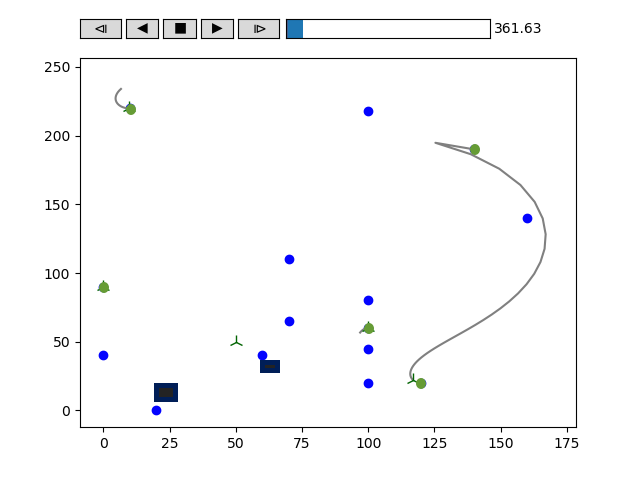
\includegraphics[width=.5\textwidth]{figs/task1.png}\hfill
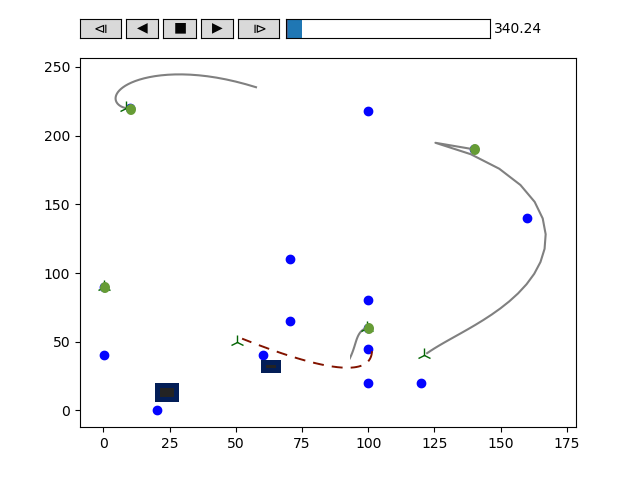
\includegraphics[width=.5\textwidth]{figs/task2.png}}\hfill%
%\includegraphics[width=.3\textwidth]{figs/Platooning_2.png}}\hfill%
\end{minipage}%
\caption{$x$ vs $y$ plots for Task App. The grey trails represent the positions of the agents in the last 150 time units, the blue dots represent the task locations of the incomplete tasks, and the green dots represent the task locations of the completed tasks. The black squares represent static obstacles. }
\label{fig:taskplots}
\end{figure}
We can also easily replace the Motion automaton (consequently, the dynamical model) of any of the agents in the program, and run the same code on them for coordinating the tasks. Using different control parameters, and path planning parameters for the same motion automaton we obtain different statistics for task completion and distance traversal as depicted in in \reffig{tasksstats}. This heterogeneity and portability can be useful for coordinating the same application between different hardware platforms.   
\begin{figure}[h!]
\begin{minipage}{0.5\textwidth}
\includegraphics[width=.5\textwidth]{figs/taskplot1.png}\hfill
\includegraphics[width=.5\textwidth]{figs/taskplot2.png}}\hfill%
%\includegraphics[width=.3\textwidth]{figs/Platooning_2.png}}\hfill%
\end{minipage}%
\caption{\small \emph{Left:} Task completion times with different configurations of agents. \emph{Right:}Min, Max and average distances travelled by each agent in different configurations.}. 
\label{fig:taskstats}
\end{figure}

 For all agents operating with the same motion automaton and dynamics model, We observed that conflict resolution took more time with more agents, as expected (\reffig{completionstats}). The completion time remained relatively stable. The maximum and minimum distances travelled were relatively closer with more robots. However, all these results were affected by the non-determinism in choice of paths and tasks by the agents, and their previous relative positions at the moment of choosing the next task as well. These results demonstrate a capability of covering various scenarios in simulation without having to incur the cost of hardware deployment.  
 
\fTBD{placeholder plot}\begin{figure}[h!]
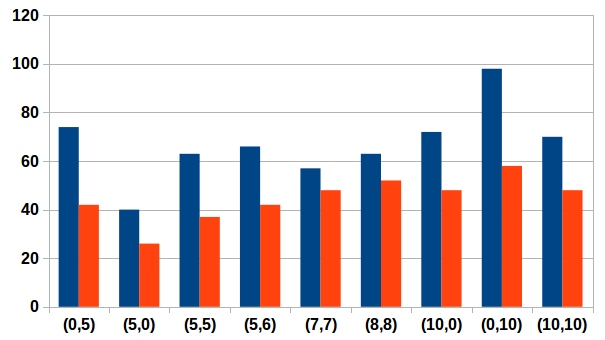
\includegraphics[width=.5\textwidth]{figs/completion.png}\hfill
\caption{\small  Blue-  total completion time and orange- time taken for conflict resolution in seconds}. 
\label{fig:taskstats}
\end{figure}